\documentclass[10pt]{article} %%%%%%%%%%%%%%%%%%%%%%%%%%%
%%%%%%%%%%%%%%%%%%%%%%%%%%%%%%%%%%%%%%%%%%%%%%%%%%%%%%%%%
%%%
%%% Apsrtable writeup for TPM, coinciding with 0.7-0
%%%
%%% mjm / 2009-01-14 %%%%%%%%%%%%%%%%%%%%%%%%%%%%%%%%%%%%


\usepackage[dvipsnames,usenames]{xcolor}
\usepackage[opticals,medfamily,minionint,footnotefigures]{MinionPro}
\usepackage[no-math]{fontspec}
\usepackage{xltxtra}
\usepackage[protrusion=true,expansion]{microtype}
%%% Hanging indents: args length, number of lines.
%%% \begin{hangparas}{1em}{1}
\usepackage{hanging} 
%%% Date formatting, defn of isodate
\usepackage{datetime}
\renewcommand{\dateseparator}{-}
\newdateformat{isodate}{%
\THEYEAR\dateseparator\twodigit{\THEMONTH}\dateseparator\twodigit{\THEDAY}}


%%% Set up bold Minion Pro math
\usepackage{bm}
 \DeclareMathAlphabet\mathbf {T1} {MinionPro-OsF}{b}{n}
 \SetMathAlphabet\mathit  {bold}{T1} {MinionPro-OsF}{b}{it}
 \SetSymbolFont{operators}{bold}{T1} {MinionPro-OsF}{b}{n}
 \SetSymbolFont{letters}  {bold}{OML}{MinionPro-TOsF} {b}{it}
\DeclareMathVersion{boldtabular}
\SetSymbolFont{operators}{boldtabular}{T1} {MinionPro-OsF}{b}{n}
\SetSymbolFont{letters}  {boldtabular}{OML}{MinionPro-TOsF}  {b}{it}
\SetMathAlphabet\mathit  {boldtabular}{T1} {MinionPro-OsF}{b}{it}
\DeclareMathAlphabet\mathebf {T1} {MinionPro-OsF}{eb}{n}

%%% PDF setup -- fill in the title
\usepackage[dvipdfm, bookmarks, colorlinks, breaklinks, pdftitle={Malecki},pdfauthor={Michael Malecki}]{hyperref}  
\hypersetup{linkcolor=NavyBlue,citecolor=NavyBlue,filecolor=NavyBlue,urlcolor=NavyBlue} 

%% Alter some LaTeX defaults for better treatment of figures:
%% This is from the first result of google: "latex dumb defaults"
    \renewcommand{\topfraction}{0.9}	
    \renewcommand{\bottomfraction}{0.8}	
    %   Parameters for TEXT pages (not float pages):
    \setcounter{topnumber}{2}
    \setcounter{bottomnumber}{2}
    \setcounter{totalnumber}{4}     
    \setcounter{dbltopnumber}{2}    
    \renewcommand{\dbltopfraction}{0.9}	
    \renewcommand{\textfraction}{0.07}	
    %   Parameters for FLOAT pages (not text pages):
    \renewcommand{\floatpagefraction}{0.7}	% require fuller float pages
	% N.B.: floatpagefraction MUST be less than topfraction !!
    \renewcommand{\dblfloatpagefraction}{0.7}	% require fuller float pages

%%% Enable the bibliography
%%%     see  http://merkel.zoneo.net/Latex/natbib.php
%%% 
%%% round: use () for in-text cites (other options square, curly, angle)
%%% sort: orders multiple citations into the sequence in which they 
%%%       appear in the list of references;
%%% sort&compress: as sort but in addition multiple numerical
%%%                citations are compressed if possible (as 3-6, 15);
%%% numbers: for numerica citations
%%% super:   superscripted numbers as in Nature
\usepackage[round]{natbib}
%%% Want to change the section head of the bib??
%\AtBeginDocument{\renewcommand\refname{LITERATURE CITED}}

%%% Document layout, margins
\usepackage{geometry} 
\geometry{letterpaper, textwidth=6.5in, textheight=8in, marginparsep=1em}

%%% This is how you set  line spacing globally inside []
%%% Options are "singlespacing","onehalfspacing","doublespacing"
%%% To change WITHIN the document (you want a section single spaced)
%%% just drop in, where needed, \singlespacing
%%% and then \doublespacing again when finished.
\usepackage[onehalfspacing]{setspace} 

%\usepackage{egameps} % See Martin Osborne's documentation!
%\usepackage{sgame} % See Osborne
%\usepackage{hyperref} % \href{http://link.com}{link text} DEF EARLIER
\usepackage{graphicx} % for figures of all kinds

%% Caption labels bold. Always left-align, do not center short ones.
%% Use . instead of : after label. Size option.
\usepackage[bf,nooneline,labelsep=period,footnotesize]{caption}
\usepackage{dcolumn}  % enable decimal align tables
%\usepackage{wrapfig}  % wrappable figures

%%% How to treat new paragraphs: units are anything that latex
%%% understands: in, mm, pt, cm, [em, ex (typographic units!)]
\setlength{\parindent}{1em} % 1em  indent first line
\setlength{\parskip}{0.5ex} % half x-height space between para

%%% Working Example of how you specify shortcut macros:
\newcommand{\ybar}{\ensuremath{\overline{y}}}

%%% Other options: Options>Soft wordwrap for easy viewing
%%% Italics and Bold: ctrl+C,F,I (C-c, C-f, C-i) for inserting italicized text. 
%%% CFB for bold.
%%% rm sf tt md bf up it sl sc 
%%% Drag citations from Bibdesk
%%% single - for intraword hyphen. Anything longer, use two -- or three ---

%%% Figures. Wrapfigure at Right Left or Center.
%%% Set bounding box size (same as figure size).
%%% Insert your figure BEFORE the text. 
%%% Subsequent text will wrap around the figure.

%%% Normally, just use figure environment.
%%% To insert a figure, drag the icon (without typing the command!) 
%%% from the finder and it will insert.
%%% Type width= or height= in the [options] before the {argument}.
%%% Latex>Insert Envt>Figure (figure* means no number)
%%% "Figure #." is handled by latex, not you. Just type.
%%% To refer to a figure (or any \label) type \ref{thelabel}
%%% in text or use Ref menu, "C-c )" emacs will do it for you.



%%% FONTS

% converts LaTeX specials (``quotes'' --- dashes etc.) to unicode
\defaultfontfeatures{Ligatures={Common}} 
%\setromanfont [Mapping=tex-text,Ligatures={Common}, BoldFont={* Bold}, ItalicFont={* Italic}]{Gentium Book Basic}
\setmainfont [Mapping=tex-text,Ligatures={Common},BoldFont={ElectraLH-Bold},ItalicFont={ElectraLH-CursiveOsF},BoldItalicFont={ElectraLH-BoldCursiveOsF},SmallCapsFont={ElectraLH-RegularSC}]{ElectraLH-RegularOsF}
\setsansfont[Mapping=tex-text,BoldFont={Delicious-Bold},ItalicFont={Delicious-Italic},SmallCapsFont={Delicious-SmallCaps}] {Delicious-Roman}
\setmonofont[Scale=0.8]{Monaco} 
%%% Section headings
\usepackage{sectsty} 
\usepackage[normalem]{ulem} 
\sectionfont{\sffamily\mdseries\upshape\Large}
\subsectionfont{\sffamily\bfseries\upshape\normalsize} 
\subsubsectionfont{\sffamily\mdseries\upshape\normalsize} 
%%% Hang section numbers in the left margin
\makeatletter 
\def\@seccntformat#1{\protect\makebox[0pt][r]{\csname 
the#1\endcsname\quad}} 
\makeatother 
\usepackage{Sweave}
%\VignetteIndexEntry{Using and Extending apsrtable}
\begin{document}

\title{Replicable Publication-Ready Model Output with R package apsrtable\\Implementation \& Extension Guide}
\author{\href{http://malecki.wustl.edu}{Michael Malecki}\footnote{PhD Candidate, Washington University in St. Louis}}
\maketitle

\section{Overview}
\label{sec:overview}

Formatting fitted model objects is not trivial and should not be done at the last minute before submitting a paper. It is too easy for modeling details to get lost, or simply for values to be omitted, transposed, or otherwise misplaced. Thus automation is a boon, if not a requirement, for replicability.

Fitted model objects in R contain a lot of information, but often we want to look at several of them side-by-side. It would be nice to name the models, and include some model-fit information, and to name the covariates. Nested and non-nested models and naming become a problem for cbind and rbind, and last but not least, we want this information in some legible format -- either plain text or, prefereably, Latex. My R package \textit{apsrtable}, installable from \href{http://cran.r-project.org/web/packages/apsrtable/index.html}{CRAN}, seeks to solve all of these problems, creating tables ready to be published in the \textit{APSR}. I might have named it after \textit{Political Analysis}, but the latter often features other innovative presentations of data and results, such that ``a \textit{PA}-style table'' is less identifiable.

Like many graduate students -- including probably most who read TPM -- I have typeset \emph{a lot} of fitted models in the course of methods training, leaving aside the relatively few tables that make their way into final seminar, conference, or journal papers. We were ``strongly encouraged'' to prepare homework assignments using Latex and create ``professional-looking'' tables of model output, with the expectation that we would get faster at it, while becoming attuned to the intricacies of Latex's tabular and matrix environments. I found this exercise as tedious as formatting a bibliography by hand. So, I set out to automate R's output of ``professional-looking'' tables. To complete the bibliography analogy, I also wanted to make the automated solution more user-friendly than bibtex BSTs -- though ``an order of magnitude easier than BST'' is still an extremely low target.

\section{Usage}
\label{sec:usage}

To demonstrate \texttt{apsrtable}'s features, I'll replicate some of the results from Persson and Tabellini's (2003) \textit{The Economic Effects of Constitutions}\footnote{The data are available from the \href{http://www.igier.unibocconi.it/whos.php?vedi=1169&tbn=albero&id_folder=177}{authors}, though they may contain some coding errors in the institutional interaction variables. A corrected replication dataset is available \href{http://malecki.wustl.edu/pt.csv}{here}.}, in particular models 1--3 of Table 6.1 (p.~159) (Figure \ref{fig:ptimage}).
\begin{figure}[htb]
  \centering
  \caption{Persson and Tabellini (2003), p.159, detail.}
  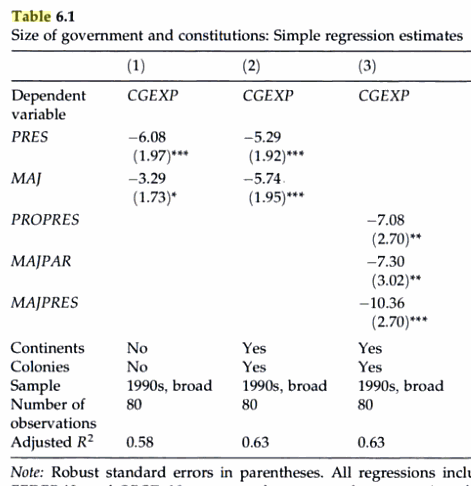
\includegraphics[width=8cm]{pt-table.png}
  \label{fig:ptimage}
\end{figure}

\begin{Schunk}
\begin{Sinput}
> pt <- read.csv("pt.csv")